% Options for packages loaded elsewhere
\PassOptionsToPackage{unicode}{hyperref}
\PassOptionsToPackage{hyphens}{url}
%
\documentclass[
]{article}
\usepackage{lmodern}
\usepackage{amsmath}
\usepackage{ifxetex,ifluatex}
\ifnum 0\ifxetex 1\fi\ifluatex 1\fi=0 % if pdftex
  \usepackage[T1]{fontenc}
  \usepackage[utf8]{inputenc}
  \usepackage{textcomp} % provide euro and other symbols
  \usepackage{amssymb}
\else % if luatex or xetex
  \usepackage{unicode-math}
  \defaultfontfeatures{Scale=MatchLowercase}
  \defaultfontfeatures[\rmfamily]{Ligatures=TeX,Scale=1}
\fi
% Use upquote if available, for straight quotes in verbatim environments
\IfFileExists{upquote.sty}{\usepackage{upquote}}{}
\IfFileExists{microtype.sty}{% use microtype if available
  \usepackage[]{microtype}
  \UseMicrotypeSet[protrusion]{basicmath} % disable protrusion for tt fonts
}{}
\makeatletter
\@ifundefined{KOMAClassName}{% if non-KOMA class
  \IfFileExists{parskip.sty}{%
    \usepackage{parskip}
  }{% else
    \setlength{\parindent}{0pt}
    \setlength{\parskip}{6pt plus 2pt minus 1pt}}
}{% if KOMA class
  \KOMAoptions{parskip=half}}
\makeatother
\usepackage{xcolor}
\IfFileExists{xurl.sty}{\usepackage{xurl}}{} % add URL line breaks if available
\IfFileExists{bookmark.sty}{\usepackage{bookmark}}{\usepackage{hyperref}}
\hypersetup{
  pdftitle={homework\_1.R},
  pdfauthor={mojmir},
  hidelinks,
  pdfcreator={LaTeX via pandoc}}
\urlstyle{same} % disable monospaced font for URLs
\usepackage[margin=1in]{geometry}
\usepackage{color}
\usepackage{fancyvrb}
\newcommand{\VerbBar}{|}
\newcommand{\VERB}{\Verb[commandchars=\\\{\}]}
\DefineVerbatimEnvironment{Highlighting}{Verbatim}{commandchars=\\\{\}}
% Add ',fontsize=\small' for more characters per line
\usepackage{framed}
\definecolor{shadecolor}{RGB}{248,248,248}
\newenvironment{Shaded}{\begin{snugshade}}{\end{snugshade}}
\newcommand{\AlertTok}[1]{\textcolor[rgb]{0.94,0.16,0.16}{#1}}
\newcommand{\AnnotationTok}[1]{\textcolor[rgb]{0.56,0.35,0.01}{\textbf{\textit{#1}}}}
\newcommand{\AttributeTok}[1]{\textcolor[rgb]{0.77,0.63,0.00}{#1}}
\newcommand{\BaseNTok}[1]{\textcolor[rgb]{0.00,0.00,0.81}{#1}}
\newcommand{\BuiltInTok}[1]{#1}
\newcommand{\CharTok}[1]{\textcolor[rgb]{0.31,0.60,0.02}{#1}}
\newcommand{\CommentTok}[1]{\textcolor[rgb]{0.56,0.35,0.01}{\textit{#1}}}
\newcommand{\CommentVarTok}[1]{\textcolor[rgb]{0.56,0.35,0.01}{\textbf{\textit{#1}}}}
\newcommand{\ConstantTok}[1]{\textcolor[rgb]{0.00,0.00,0.00}{#1}}
\newcommand{\ControlFlowTok}[1]{\textcolor[rgb]{0.13,0.29,0.53}{\textbf{#1}}}
\newcommand{\DataTypeTok}[1]{\textcolor[rgb]{0.13,0.29,0.53}{#1}}
\newcommand{\DecValTok}[1]{\textcolor[rgb]{0.00,0.00,0.81}{#1}}
\newcommand{\DocumentationTok}[1]{\textcolor[rgb]{0.56,0.35,0.01}{\textbf{\textit{#1}}}}
\newcommand{\ErrorTok}[1]{\textcolor[rgb]{0.64,0.00,0.00}{\textbf{#1}}}
\newcommand{\ExtensionTok}[1]{#1}
\newcommand{\FloatTok}[1]{\textcolor[rgb]{0.00,0.00,0.81}{#1}}
\newcommand{\FunctionTok}[1]{\textcolor[rgb]{0.00,0.00,0.00}{#1}}
\newcommand{\ImportTok}[1]{#1}
\newcommand{\InformationTok}[1]{\textcolor[rgb]{0.56,0.35,0.01}{\textbf{\textit{#1}}}}
\newcommand{\KeywordTok}[1]{\textcolor[rgb]{0.13,0.29,0.53}{\textbf{#1}}}
\newcommand{\NormalTok}[1]{#1}
\newcommand{\OperatorTok}[1]{\textcolor[rgb]{0.81,0.36,0.00}{\textbf{#1}}}
\newcommand{\OtherTok}[1]{\textcolor[rgb]{0.56,0.35,0.01}{#1}}
\newcommand{\PreprocessorTok}[1]{\textcolor[rgb]{0.56,0.35,0.01}{\textit{#1}}}
\newcommand{\RegionMarkerTok}[1]{#1}
\newcommand{\SpecialCharTok}[1]{\textcolor[rgb]{0.00,0.00,0.00}{#1}}
\newcommand{\SpecialStringTok}[1]{\textcolor[rgb]{0.31,0.60,0.02}{#1}}
\newcommand{\StringTok}[1]{\textcolor[rgb]{0.31,0.60,0.02}{#1}}
\newcommand{\VariableTok}[1]{\textcolor[rgb]{0.00,0.00,0.00}{#1}}
\newcommand{\VerbatimStringTok}[1]{\textcolor[rgb]{0.31,0.60,0.02}{#1}}
\newcommand{\WarningTok}[1]{\textcolor[rgb]{0.56,0.35,0.01}{\textbf{\textit{#1}}}}
\usepackage{graphicx}
\makeatletter
\def\maxwidth{\ifdim\Gin@nat@width>\linewidth\linewidth\else\Gin@nat@width\fi}
\def\maxheight{\ifdim\Gin@nat@height>\textheight\textheight\else\Gin@nat@height\fi}
\makeatother
% Scale images if necessary, so that they will not overflow the page
% margins by default, and it is still possible to overwrite the defaults
% using explicit options in \includegraphics[width, height, ...]{}
\setkeys{Gin}{width=\maxwidth,height=\maxheight,keepaspectratio}
% Set default figure placement to htbp
\makeatletter
\def\fps@figure{htbp}
\makeatother
\setlength{\emergencystretch}{3em} % prevent overfull lines
\providecommand{\tightlist}{%
  \setlength{\itemsep}{0pt}\setlength{\parskip}{0pt}}
\setcounter{secnumdepth}{-\maxdimen} % remove section numbering
\ifluatex
  \usepackage{selnolig}  % disable illegal ligatures
\fi

\title{homework\_1.R}
\author{mojmir}
\date{2020-12-10}

\begin{document}
\maketitle

\begin{Shaded}
\begin{Highlighting}[]
\FunctionTok{library}\NormalTok{(janeaustenr)}
\FunctionTok{library}\NormalTok{(dplyr)}
\FunctionTok{library}\NormalTok{(stringr)}

\NormalTok{original\_books }\OtherTok{\textless{}{-}} \FunctionTok{austen\_books}\NormalTok{() }\SpecialCharTok{\%\textgreater{}\%}
  \FunctionTok{group\_by}\NormalTok{(book) }\SpecialCharTok{\%\textgreater{}\%}
  \FunctionTok{mutate}\NormalTok{(}\AttributeTok{linenumber =} \FunctionTok{row\_number}\NormalTok{(),}
         \AttributeTok{chapter =} \FunctionTok{cumsum}\NormalTok{(}\FunctionTok{str\_detect}\NormalTok{(text, }\FunctionTok{regex}\NormalTok{(}\StringTok{"\^{}chapter [}\SpecialCharTok{\textbackslash{}\textbackslash{}}\StringTok{divxlc]"}\NormalTok{,}
                                                 \AttributeTok{ignore\_case =} \ConstantTok{TRUE}\NormalTok{)))) }\SpecialCharTok{\%\textgreater{}\%}
  \FunctionTok{ungroup}\NormalTok{()}

\NormalTok{original\_books}
\end{Highlighting}
\end{Shaded}

\begin{verbatim}
## # A tibble: 73,422 x 4
##    text                    book                linenumber chapter
##    <chr>                   <fct>                    <int>   <int>
##  1 "SENSE AND SENSIBILITY" Sense & Sensibility          1       0
##  2 ""                      Sense & Sensibility          2       0
##  3 "by Jane Austen"        Sense & Sensibility          3       0
##  4 ""                      Sense & Sensibility          4       0
##  5 "(1811)"                Sense & Sensibility          5       0
##  6 ""                      Sense & Sensibility          6       0
##  7 ""                      Sense & Sensibility          7       0
##  8 ""                      Sense & Sensibility          8       0
##  9 ""                      Sense & Sensibility          9       0
## 10 "CHAPTER 1"             Sense & Sensibility         10       1
## # ... with 73,412 more rows
\end{verbatim}

\begin{Shaded}
\begin{Highlighting}[]
\FunctionTok{library}\NormalTok{(tidytext)}
\NormalTok{tidy\_books }\OtherTok{\textless{}{-}}\NormalTok{ original\_books }\SpecialCharTok{\%\textgreater{}\%}
  \FunctionTok{unnest\_tokens}\NormalTok{(word, text)}

\NormalTok{tidy\_books}
\end{Highlighting}
\end{Shaded}

\begin{verbatim}
## # A tibble: 725,055 x 4
##    book                linenumber chapter word       
##    <fct>                    <int>   <int> <chr>      
##  1 Sense & Sensibility          1       0 sense      
##  2 Sense & Sensibility          1       0 and        
##  3 Sense & Sensibility          1       0 sensibility
##  4 Sense & Sensibility          3       0 by         
##  5 Sense & Sensibility          3       0 jane       
##  6 Sense & Sensibility          3       0 austen     
##  7 Sense & Sensibility          5       0 1811       
##  8 Sense & Sensibility         10       1 chapter    
##  9 Sense & Sensibility         10       1 1          
## 10 Sense & Sensibility         13       1 the        
## # ... with 725,045 more rows
\end{verbatim}

\begin{Shaded}
\begin{Highlighting}[]
\FunctionTok{data}\NormalTok{(stop\_words)}

\NormalTok{tidy\_books }\OtherTok{\textless{}{-}}\NormalTok{ tidy\_books }\SpecialCharTok{\%\textgreater{}\%}
  \FunctionTok{anti\_join}\NormalTok{(stop\_words)}
\end{Highlighting}
\end{Shaded}

\begin{Shaded}
\begin{Highlighting}[]
\NormalTok{tidy\_books }\SpecialCharTok{\%\textgreater{}\%}
  \FunctionTok{count}\NormalTok{(word, }\AttributeTok{sort =} \ConstantTok{TRUE}\NormalTok{)}
\end{Highlighting}
\end{Shaded}

\begin{verbatim}
## # A tibble: 13,914 x 2
##    word       n
##    <chr>  <int>
##  1 miss    1855
##  2 time    1337
##  3 fanny    862
##  4 dear     822
##  5 lady     817
##  6 sir      806
##  7 day      797
##  8 emma     787
##  9 sister   727
## 10 house    699
## # ... with 13,904 more rows
\end{verbatim}

\begin{Shaded}
\begin{Highlighting}[]
\FunctionTok{library}\NormalTok{(ggplot2)}

\NormalTok{tidy\_books }\SpecialCharTok{\%\textgreater{}\%}
  \FunctionTok{count}\NormalTok{(word, }\AttributeTok{sort =} \ConstantTok{TRUE}\NormalTok{) }\SpecialCharTok{\%\textgreater{}\%}
  \FunctionTok{filter}\NormalTok{(n }\SpecialCharTok{\textgreater{}} \DecValTok{600}\NormalTok{) }\SpecialCharTok{\%\textgreater{}\%}
  \FunctionTok{mutate}\NormalTok{(}\AttributeTok{word =} \FunctionTok{reorder}\NormalTok{(word, n)) }\SpecialCharTok{\%\textgreater{}\%}
  \FunctionTok{ggplot}\NormalTok{(}\FunctionTok{aes}\NormalTok{(word, n)) }\SpecialCharTok{+}
  \FunctionTok{geom\_col}\NormalTok{() }\SpecialCharTok{+}
  \FunctionTok{xlab}\NormalTok{(}\ConstantTok{NULL}\NormalTok{) }\SpecialCharTok{+}
  \FunctionTok{coord\_flip}\NormalTok{()}
\end{Highlighting}
\end{Shaded}

\begin{figure}
\centering
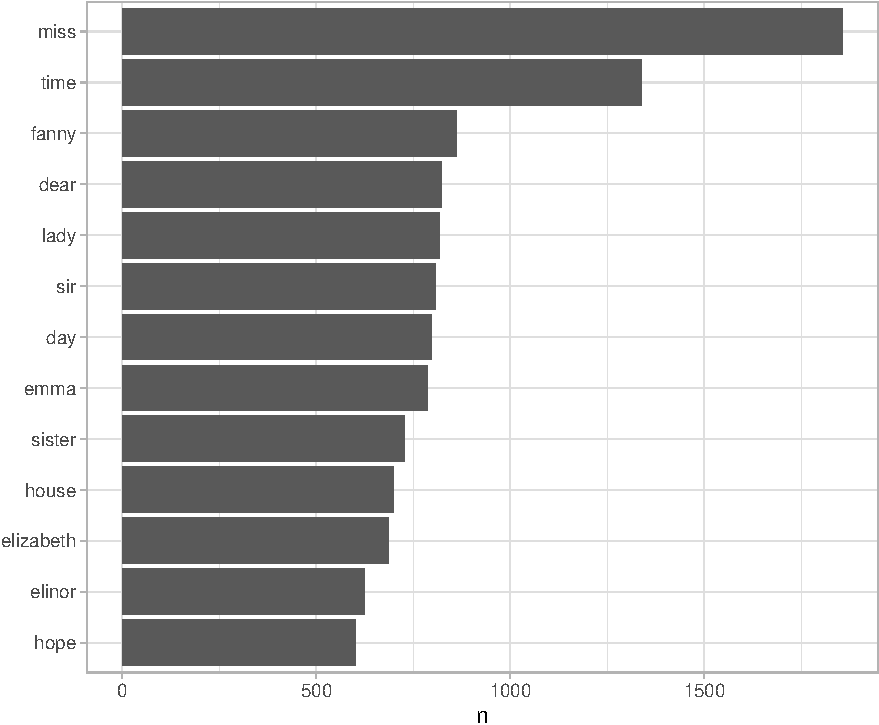
\includegraphics{homework_1_files/figure-latex/plotcount-1.pdf}
\caption{The most common words in Jane Austen's novels}
\end{figure}

\begin{Shaded}
\begin{Highlighting}[]
\CommentTok{\# the same but with gutenberg download}
\DocumentationTok{\#\# To learn more about gutenbergr, check out the [package\textquotesingle{}s tutorial at rOpenSci](https://ropensci.org/tutorials/gutenbergr\_tutorial.html), where it is one of rOpenSci\textquotesingle{}s packages for data access.}
\end{Highlighting}
\end{Shaded}

\begin{Shaded}
\begin{Highlighting}[]
\FunctionTok{library}\NormalTok{(gutenbergr)}

\DocumentationTok{\#\# Own example: Alice}

\NormalTok{alice }\OtherTok{\textless{}{-}} \FunctionTok{gutenberg\_download}\NormalTok{(}\DecValTok{11}\NormalTok{)}

\NormalTok{tidy\_alice }\OtherTok{\textless{}{-}}\NormalTok{ alice }\SpecialCharTok{\%\textgreater{}\%}
  \FunctionTok{unnest\_tokens}\NormalTok{(word, text) }\SpecialCharTok{\%\textgreater{}\%}
  \FunctionTok{anti\_join}\NormalTok{(stop\_words)}

\NormalTok{tidy\_alice }\SpecialCharTok{\%\textgreater{}\%}
  \FunctionTok{count}\NormalTok{(word, }\AttributeTok{sort =} \ConstantTok{TRUE}\NormalTok{)}
\end{Highlighting}
\end{Shaded}

\begin{verbatim}
## # A tibble: 2,322 x 2
##    word        n
##    <chr>   <int>
##  1 alice     386
##  2 time       71
##  3 queen      68
##  4 king       61
##  5 don’t      60
##  6 it’s       57
##  7 mock       57
##  8 i’m        56
##  9 turtle     56
## 10 gryphon    55
## # ... with 2,312 more rows
\end{verbatim}

\begin{Shaded}
\begin{Highlighting}[]
\FunctionTok{library}\NormalTok{(ggplot2)}


\NormalTok{tidy\_alice }\SpecialCharTok{\%\textgreater{}\%}
  \FunctionTok{count}\NormalTok{(word, }\AttributeTok{sort =} \ConstantTok{TRUE}\NormalTok{) }\SpecialCharTok{\%\textgreater{}\%}
  \FunctionTok{filter}\NormalTok{(n }\SpecialCharTok{\textgreater{}} \DecValTok{50}\NormalTok{) }\SpecialCharTok{\%\textgreater{}\%}
  \FunctionTok{mutate}\NormalTok{(}\AttributeTok{word =} \FunctionTok{reorder}\NormalTok{(word, n)) }\SpecialCharTok{\%\textgreater{}\%}
  \FunctionTok{ggplot}\NormalTok{(}\FunctionTok{aes}\NormalTok{(word, n)) }\SpecialCharTok{+}
  \FunctionTok{geom\_col}\NormalTok{() }\SpecialCharTok{+}
  \FunctionTok{xlab}\NormalTok{(}\ConstantTok{NULL}\NormalTok{) }\SpecialCharTok{+}
  \FunctionTok{coord\_flip}\NormalTok{() }\SpecialCharTok{+}
  \FunctionTok{ggtitle}\NormalTok{(}\StringTok{"Alice: most common words"}\NormalTok{)}
\end{Highlighting}
\end{Shaded}

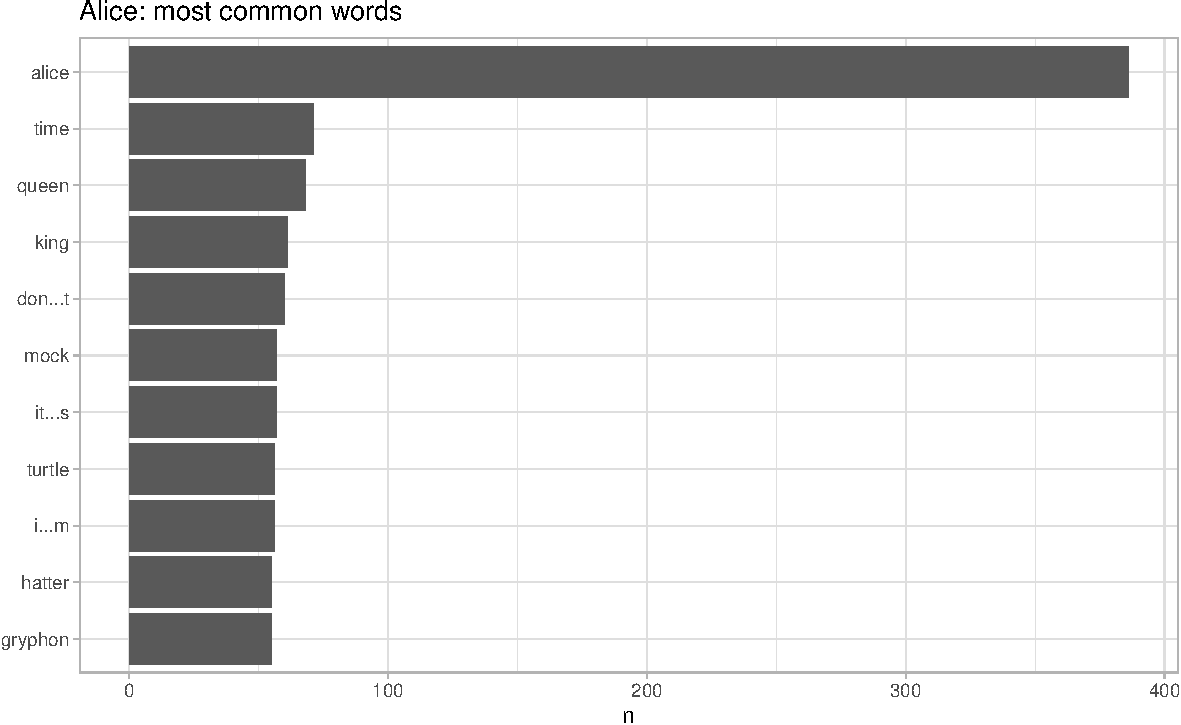
\includegraphics{homework_1_files/figure-latex/unnamed-chunk-2-1.pdf}

\end{document}
